\chapter{結果と考察}
\label{CResult}

%% \textcolor{red}{****メモ始め****}
%% \begin{itemize}
%% \item 使用したテクスチャとかの画像を載せる
%% \item 形状モデルのワイヤフレーム画像
%% \item ポリゴン数とか面の数、頂点の数でテーブルを作成する
%% \item 球がひとつの場合の実物との比較
%% \item 平面オブジェクトに対する実行結果と解像度$R_t$の評価
%% \item 球体オブジェクト
%% \item 実行結果の処理速度のグラフを作る
%% \item 結果の実物との比較
%% \item 定性的評価
%% \item さまざまなオブジェクトへの適用
%% \item 鹿児島アートフェスタ
%% \end{itemize}
%% \textcolor{red}{****メモ終わり****}

\section{実装方法および実行環境}
\label{SEnvironment}

本手法ではグラフィックスライブラリとしてOpenGL(オープンジーエル: Open Graphics Library)を利用し、プログラムの実装にあたってはC++言語を用いている。
GPU上で動作するプログラムの実装にあたっては、GLSL(ジーエルエスエル: OpenGL Shading Language)を用いた。
本手法を適用する形状データはAutodesk Mayaで作成したオブジェクトファイルを使って作成した。

プログラムの実行に使用した計算機のハードウェア構成は\tabref{tab:experiment-hadrware}のとおりである。

\begin{table}
\centering
\caption{実行環境 \label{tab:experiment-hadrware}}
\begin{tabular}{r|l}
\hline
CPU & Intel Core i7 960 3.20 GHz \\ \hline
メモリ & 30 GB \\ \hline
GPU & NVIDIA GeForce GTX 660 \\ \hline
%グラフィックメモリ & 3 GB GDDR5 \\ \hline
\end{tabular}
\end{table}

%------------------------------------------------------------------------------------------
\section{処理系}
\label{S}

\subsection{内部通過処理および外部通過処理}
\label{SSInnerOuterProcess}

\chapref{CMethod}で述べた隣接球を通過する光の挙動について、平面オブジェクトおよび球体オブジェクトを例に問題点を指摘する。
%% 本手法で用いた複眼の近似モデル(\secref{SSModel})では、個眼のレンズの代わりに球体レンズを利用している。
%% また、本来は予備実験\secref{SSMarbleOnHole}のように最密に球を配置することが理想であるが、本手法では評価実験のためにアルゴリズムが簡略な格子状の配置を採択している。**methodに追記する**
本手法では、球体レンズ同士の間にできる隙間を埋めるために、球の直径を球同士の中心距離よりも大きく設定している(\secref{SSMultiRefraction})。
また、複数の球を通過する光を想定し、光が球の外部を経由して隣接する球に入射する場合のアルゴリズムを実装していた。
しかし、外部を経由する場合の実装(以下、外部通過処理)によって得られる結果画像にはノイズが多く、求める画像とは異なる結果となってしまった\figref{FNoise}。
\begin{figure}[htbp]
  \centering
\subfigure[平面オブジェクト]{
\includegraphics*[width=.45\columnwidth]{./img/screenshot/sphere/Noise/pscreenshot005.bmp}
\label{FNoisePlane}}
\subfigure[球体オブジェクト]{
\includegraphics*[width=.45\columnwidth]{./img/screenshot/sphere/Noise/screenshot000.bmp}
\label{FNoiseSphere}}
  \caption{外部通過処理に見られるノイズ}
  \label{FNoise}
\end{figure}
そのため、手法の修正として外部通過処理を実装から排除し、球の内部から内部への光の通過を考慮した実装(以下、内部通過処理)のみを採択することにした。

外部通過処理を排除しても、本手法で想定される範囲内では問題はないと考えられる。
理由として、外部通過処理と内部通過処理のそれぞれによって得られる画像にはノイズの有無以外に大きな差異が観測されなかったことと、球の半径を十分に大きい値で設定すれば、球の外部を経由して隣接する球に入射する光はあまり存在しないと推測されることが挙げられる。
ゆえに、本章での考察は主に内部通過処理によって得られるものに対して行う。

%------------------------------------------------------------------------------------------

\section{ジオメトリ}
\label{S}

\subsection{レンズ半径と偽瞳孔の数}
\label{SS}

本手法では、レンズの位置座標とレンズの半径は独立して扱うことができる。
\secref{SSInnerOuterProcess}でも述べたように、本手法では配置された球体レンズ同士の間の隙間を埋めるため、球の半径を球同士が接するよりも大きい値で設定しており、球の半径によって光の入射する領域のレンズの曲率が変化する。
すなわち、球の半径$r$の設定値によって複眼の外観が変化するため、両者の関係について考察を行う。
以下ではテクスチャに後述の\figref{FBaseTexture}を使用しており、テクスチャ解像度$R_t = 300$を使用している。
ここでは、入力したオブジェクトファイルのうち平面オブジェクトの1辺のながさとテクスチャの距離$1$が、球体オブジェクトに関しては大円の長さとテクスチャの距離$1$とが対応している。

\begin{figure}[htbp]
  \centering
\subfigure[$r = 0.03$]{
\includegraphics*[width=.3\columnwidth]{./img/screenshot/sphere/Radius/1_30/screenshot000.bmp}
\label{FRadius003-0}}
\subfigure[$r = 0.03$]{
\includegraphics*[width=.3\columnwidth]{./img/screenshot/sphere/Radius/1_30/screenshot001.bmp}
\label{FRadius003-1}}
\subfigure[$r = 0.03$]{
\includegraphics*[width=.3\columnwidth]{./img/screenshot/sphere/Radius/1_30/screenshot002.bmp}
\label{FRadius003-2}}\\
\subfigure[$r = 0.04$]{
\includegraphics*[width=.3\columnwidth]{./img/screenshot/sphere/Radius/1_24/screenshot000.bmp}
\label{FRadius004-0}}
\subfigure[$r = 0.04$]{
\includegraphics*[width=.3\columnwidth]{./img/screenshot/sphere/Radius/1_24/screenshot001.bmp}
\label{FRadius004-1}}
\subfigure[$r = 0.04$]{
\includegraphics*[width=.3\columnwidth]{./img/screenshot/sphere/Radius/1_24/screenshot002.bmp}
\label{FRadius004-2}}\\
\subfigure[$r = 0.06$]{
\includegraphics*[width=.3\columnwidth]{./img/screenshot/sphere/Radius/1_16/screenshot000.bmp}
\label{FRadius006-0}}
\subfigure[$r = 0.06$]{
\includegraphics*[width=.3\columnwidth]{./img/screenshot/sphere/Radius/1_16/screenshot001.bmp}
\label{FRadius006-1}}
\subfigure[$r = 0.06$]{
\includegraphics*[width=.3\columnwidth]{./img/screenshot/sphere/Radius/1_16/screenshot002.bmp}
\label{FRadius006-2}}\\
\subfigure[$r = 0.10$]{
\includegraphics*[width=.3\columnwidth]{./img/screenshot/sphere/Radius/1_10/screenshot000.bmp}
\label{FRadius010-0}}
\subfigure[$r = 0.10$]{
\includegraphics*[width=.3\columnwidth]{./img/screenshot/sphere/Radius/1_10/screenshot001.bmp}
\label{FRadius010-1}}
\subfigure[$r = 0.10$]{
\includegraphics*[width=.3\columnwidth]{./img/screenshot/sphere/Radius/1_10/screenshot002.bmp}
\label{FRadius010-2}}
  \caption{レンズ半径$r$と偽瞳孔の数の関係}
  \label{FRadiusAndNumber}
\end{figure}

比較画像\figref{FRadiusAndNumber}からレンズ半径が大きくなるにつれて観測される偽瞳孔の数は増加していることがわかる。
これは、半径が小さく曲率が大きければ個眼の端でのレンズ表面への進入角が小さくなるので、より内側への屈折が起こり、逆に半径が大きく曲率が小さければ、進入角が相対的に大きくなるので屈折の度合いが抑えられ、結果的に隣接する色素細胞テクスチャへ到達する頻度が高くなるためであると考えられる。

生物の個眼のレンズの曲率には幅があり、ハエの一種のように曲率の大きなものからトンボやチョウのように曲率の小さいものまで存在する。
曲率の値は固定していないが、ユーザが半径値$r$を設定することで任意の曲率を表現することができる。

%% 再現性を高めるためには、対象生物の個眼のレンズの曲率を測定するか、ユーザが任意の半径値$r$を設定することが必要となるが、ある程度恣意的に結果を操作できる点はユーザビリティにつながるのではないだろうか。
%% 事実、生物種によって観察される偽瞳孔の密度や分布は異なるため、求める結果を得るための試行錯誤が必要である。


\subsection{歪みとテクスチャの関係}
\label{SSDistortion}

結果画像の一部には歪みが生じている部分が存在する\figref{FTexTortion}。
これは、オブジェクトに適用されたテクスチャに継ぎ目が存在し、なめらかに接続していないことが原因である。
本手法の特性上、曲面オブジェクトの表面に対しては格子状にテクスチャを適用する必要があるため、立体表面でテクスチャの歪みが生じることは避けられない。
すなわち、閉じた立体ではなく開いた曲面もしくはテクスチャの継ぎ目を表示しないモデルを使用するなどの工夫が要求される。
また、この問題はレンズ球の配置条件によって生じるので、レンズ球の配置アルゴリズムを改善するなどの対応策が今後求められる。

\begin{figure}[htbp]
  \centering
\subfigure[テクスチャマップ]{
\includegraphics*[width=.45\columnwidth]{./img/screenshot/sphere/Distortion/tex_tortion1.png}
\label{FTexTortion1}}
\subfigure[結果]{
\includegraphics*[width=.45\columnwidth]{./img/screenshot/sphere/Distortion/screenshot000.bmp}
\label{FTexTortion1-s}}\\
\subfigure[テクスチャマップ]{
\includegraphics*[width=.45\columnwidth]{./img/screenshot/sphere/Distortion/tex_tortion2.png}
\label{FTexTortion2}}
\subfigure[結果]{
\includegraphics*[width=.45\columnwidth]{./img/screenshot/sphere/Distortion/screenshot001.bmp}
\label{FTexTortion2-s}}\\
\subfigure[テクスチャマップ]{
\includegraphics*[width=.45\columnwidth]{./img/screenshot/sphere/Distortion/tex_tortion3.png}
\label{FTexTortion3}}
\subfigure[結果]{
\includegraphics*[width=.45\columnwidth]{./img/screenshot/sphere/Distortion/screenshot002.bmp}
\label{FTexTortion3-s}}\\
  \caption{テクスチャの継ぎ目}
  \label{FTexTortion}
\end{figure}

\newpage
\subsection{さまざまなテクスチャ}%%---done
\label{SS}

本手法ではテクスチャを変更することにより外観が大幅に変化する。
基本的には、モデルであるパンチングメタルを模して黒点のテクスチャをタイリングする。
以下に、本手法で用いた基本のテクスチャおよび任意のテクスチャを使用した場合の結果を紹介する\figref{FBaseTextureAndResult}。
基本のテクスチャは球の中心と黒点の中心を合わせる必要があるため、画像中心から同心円上に広がる黒点を使用している。
同じ黒点のテクスチャ\figref{FBaseTexture}, \figref{FTex3}であっても\figref{FBaseResult}と\figref{FTexResult3}のように、得られる結果画像は大きく異なることがわかる。
また、\figref{FTex1}, \figref{FTexResult1}および\figref{FTex2},\figref{FTexResult2}からは、敷き詰められた球体レンズによって基本となるテクスチャの画像が拡大されていることが確認できる。
よって、本手法は\secref{SExperimentResult}の結果を反映していると言える。


\begin{figure}[htbp]
  \centering
\subfigure[基本テクスチャ]{
\includegraphics*[width=.45\columnwidth]{./img/screenshot/texture/spot.jpg}
\label{FBaseTexture}}\\
\subfigure[結果画像]{
\includegraphics*[width=.45\columnwidth]{./img/screenshot/texture/spot.bmp}
\label{FBaseResult}}
  \caption{基本テクスチャと適用結果}
  \label{FBaseTextureAndResult}
\end{figure}

\newpage
\begin{figure}[htbp]
  \centering
\subfigure[テクスチャ]{
\includegraphics*[width=.3\columnwidth]{./img/screenshot/texture/a.jpg}
\label{FTex1}}
\subfigure[結果]{
\includegraphics*[width=.45\columnwidth]{./img/screenshot/texture/a.bmp}
\label{FTexResult1}}\\
\subfigure[テクスチャ]{
\includegraphics*[width=.3\columnwidth]{./img/screenshot/texture/colormap.jpg}
\label{FTex2}}
\subfigure[結果]{
\includegraphics*[width=.45\columnwidth]{./img/screenshot/texture/colormap.bmp}
\label{FTexResult2}}\\
\subfigure[テクスチャ]{
\includegraphics*[width=.3\columnwidth]{./img/screenshot/texture/spot5.jpg}
\label{FTex3}}
\subfigure[結果]{
\includegraphics*[width=.45\columnwidth]{./img/screenshot/texture/spot5.bmp}
\label{FTexResult3}}\\
  \caption{テクスチャの変更による外観の変化}
  \label{FTexResults}
\end{figure}




%------------------------------------------------------------------------------------------
\newpage
\newpage
\section{パラメータと実行速度}
\label{SParameterAndExeTime}

それぞれのパラメータに応じて得られる結果画像や実行速度について比較、検討を行う。
評価を行うパラメータは光が通過する球の数の上限値、視点との距離、個眼密度である。
カメラの垂直画角およびレンズの屈折率は固定する。
\chapref{CExperiment}でレンズとして用いたビー玉はガラス製であるため、屈折率はガラスの文献値$1.491$を用いる。
対象オブジェクトは以下に示す平面オブジェクトおよび球体オブジェクトとする。
\begin{figure}[htbp]
  \centering
\subfigure[平面オブジェクト(ワイヤフレーム)]{
\includegraphics*[width=.45\columnwidth]{./img/screenshot/plane_wireframe.png}
\label{FNoisePlane}}
\subfigure[球体オブジェクト(ワイヤフレーム)]{
\includegraphics*[width=.45\columnwidth]{./img/screenshot/sphere_wireframe.png}
\label{FNoiseSphere}}
  \caption{評価オブジェクト(ワイヤフレーム表示)}
  \label{FEvalObject}
\end{figure}

\begin{table}[htbp]
\centering
\caption{オブジェクト情報 \label{TObjectInfo}}
\begin{tabular}{r||l|l|}
\hline
 & 平面オブジェクト & 球体オブジェクト \\ \hline
頂点数 & 4 & 9218 \\ \hline
面の数 & 2 & 18432 \\ \hline
ポリゴンの種類 & 三角形 & 三角形 \\ \hline
%グラフィックメモリ & 3 GB GDDR5 \\ \hline
\end{tabular}
\end{table}

\subsection{隣接球の処理ON/OFF}%%---done
\label{SSLimitNeighborSphere}

光がどの程度の回数、隣接球を通過する必要があるのかについての考察を行う。
光が複眼表面に対して平行に近い角度で入射した場合、光はひとつの球だけではなくふたつ以上の球を通過すると考えられる。
通過する球の数が増えればそれだけ処理に時間がかかるため、通過する球の数には上限値を設定する必要がある。
すなわち、物理的な正確さと処理速度はトレードオフの関係にあると言える。

では、通過する球の数の上限値を変化させることによって得られる結果について議論を行う。
上限値を設定することによる操作をここでは隣接球処理と呼ぶことにする。
以下では上限値$l = 0,1,2,3, ......$のように設定し、上限値$l$が$0$の場合には隣接球処理を行わないこととする。
すなわち、$l = 0$の場合、最初の球に入射した光は他のいかなる隣接球にも入射せずテクスチャ平面(\secref{SSModel})へ到達するものとして考える。
以下にまず、各$l$の値に対する結果を示す\figref{FLimitCompare1}\figref{FLimitCompare2}。
テクスチャは\figref{FBaseTexture}を使用しており、球の半径$r$の値は約$3.3 \times 10^{-2}$、テクスチャ解像度$R_t = 300$を使用している。

\begin{figure}[htbp]
  \centering
\subfigure[$l = 0$]{
\includegraphics*[width=.45\columnwidth]{./img/screenshot/sphere/RefracLimit/000/screenshot002.bmp}
\label{FLimit0-4}}
\subfigure[$l = 1$]{
\includegraphics*[width=.45\columnwidth]{./img/screenshot/sphere/RefracLimit/001/screenshot002.bmp}
\label{FLimit1-4}}\\
\subfigure[$l = 2$]{
\includegraphics*[width=.45\columnwidth]{./img/screenshot/sphere/RefracLimit/002/screenshot002.bmp}
\label{FLimit2-4}}
\subfigure[$l = 3$]{
\includegraphics*[width=.45\columnwidth]{./img/screenshot/sphere/RefracLimit/003/screenshot002.bmp}
\label{FLimit3-4}}\\
\subfigure[$l = 5$]{
\includegraphics*[width=.45\columnwidth]{./img/screenshot/sphere/RefracLimit/005/screenshot002.bmp}
\label{FLimit5-4}}
\subfigure[$l = 10$]{
\includegraphics*[width=.45\columnwidth]{./img/screenshot/sphere/RefracLimit/010/screenshot002.bmp}
\label{FLimit10-4}}
  \caption{上限値による画像の変化1}
  \label{FLimitCompare1}
\end{figure}

\begin{figure}[htbp]
  \centering
\subfigure[$l = 0$]{
\includegraphics*[width=.45\columnwidth]{./img/screenshot/sphere/RefracLimit/000/screenshot001.bmp}
\label{FLimit0-3}}
\subfigure[$l = 1$]{
\includegraphics*[width=.45\columnwidth]{./img/screenshot/sphere/RefracLimit/001/screenshot001.bmp}
\label{FLimit1-3}}\\
\subfigure[$l = 2$]{
\includegraphics*[width=.45\columnwidth]{./img/screenshot/sphere/RefracLimit/002/screenshot001.bmp}
\label{FLimit2-3}}
\subfigure[$l = 3$]{
\includegraphics*[width=.45\columnwidth]{./img/screenshot/sphere/RefracLimit/003/screenshot001.bmp}
\label{FLimit3-3}}\\
\subfigure[$l = 5$]{
\includegraphics*[width=.45\columnwidth]{./img/screenshot/sphere/RefracLimit/005/screenshot001.bmp}
\label{FLimit5-3}}
\subfigure[$l = 10$]{
\includegraphics*[width=.45\columnwidth]{./img/screenshot/sphere/RefracLimit/010/screenshot001.bmp}
\label{FLimit10-3}}\\
  \caption{上限値による画像の変化2}
  \label{FLimitCompare2}
\end{figure}



\newpage
結果画像からは$l = 0$の場合とそれ以外とで顕著な差異が見られ、$l = 1$および$l = 2$の場合とそれ以外の場合でわずかな差異が確認できた。
また、$l = 3$以上の場合については肉眼で判別できるほどの差異は見つからなかった。
まず、$l = 0$の場合とそれ以外との差異について述べる。
$l = 0$の場合、side pupil(\secref{SSSidePupil})の存在が確認できるものの、他の場合と比較するとやや黒色が薄く、隣接球処理をした場合のほうがはっきりとしたside pupilとなっていることがわかる。
\begin{figure}[htbp]
  \centering
\subfigure[$l = 1$]{
\includegraphics*[width=.75\columnwidth]{./img/screenshot/sphere/RefracLimit/001/pupil4_explain.png}
\label{FPupil4}}\\
\subfigure[$l = 1$]{
\includegraphics*[width=.75\columnwidth]{./img/screenshot/sphere/RefracLimit/001/pupil3_explain.png}
\label{FPupil3}}
  \caption{各偽瞳孔の名称および場所}
  \label{FPseudopupilName}
\end{figure}
$l = 1,2$の場合とそれ以外の場合を代表して$l = 3$の場合について比較を行うと、球体オブジェクトの縁において有意差が見られる。
$l = 1$の場合、side pupilのさらに外側に位置するsecond side pupil(\figref{FLimitCompare3}\figref{FLimitCompare4}緑部)のあたりは$l = 3$の場合よりも黒点の形状が曖昧となっている。
逆に、$l = 2$の場合は$l = 1,3$の場合と比較して白色領域が広くなっている。
特に、$l = 1$の場合では\figref{FLimitCompare3}\figref{FLimitCompare4}黄部付近のsecond side pupilがやや大きいのに対して、それ以降の場合では縮小していることが顕著に観測される。
以上のことから、偽瞳孔のside pupilおよびsecond side pupilには隣接球を通過する光が影響していることがわかり、\secref{SSSidePupil}の理論と一致する。

続いて、実行速度と$l$の関係を示す\figref{FExetimeAndL}。
\begin{figure}[htbp]
  \centering
\subfigure[平均値]{
\includegraphics*[width=.75\columnwidth]{./img/graph/exetime_average.png}
\label{FExetimeAverage}}\\
\subfigure[実測値]{
\includegraphics*[width=.75\columnwidth]{./img/graph/exetime_samp.png}
\label{FExetimeSamp}}
  \caption{実行速度と$l$の関係}
  \label{FExetimeAndL}
\end{figure}
平均値\figref{FExetimeAverage}と実測値\figref{FExetimeSamp}のいずれのグラフからも、実行速度と通過隣接球上限値$l$は線形の関係であることがわかる。
さらに、リアルタイムの基準が60 fpsであるとすると、今回の球体オブジェクトの場合では$l=900$付近がリアルタイムの限界値であると考えられる。
また、先述のように$l=3$以上では結果画像に有意な差が見られないことから、$l$の設定値は$10^1$オーダーで十分であると言える。

%% \textcolor{red}{実行速度と$l = 10$程度で十分とかそういう話}


\newpage
\begin{figure}[htbp]
  \centering
\subfigure[$l = 0$]{
\includegraphics*[width=.45\columnwidth]{./img/screenshot/sphere/RefracLimit/000/marker4.png}
\label{FMarker0}}
\subfigure[$l = 1$]{
\includegraphics*[width=.45\columnwidth]{./img/screenshot/sphere/RefracLimit/001/marker4.png}
\label{FMarker1}}\\
\subfigure[$l = 2$]{
\includegraphics*[width=.45\columnwidth]{./img/screenshot/sphere/RefracLimit/002/marker4.png}
\label{FMarker2}}
\subfigure[$l = 3$]{
\includegraphics*[width=.45\columnwidth]{./img/screenshot/sphere/RefracLimit/003/marker4.png}
\label{FMarker3}}\\
  \caption{上限値による画像の変化比較3}
  \label{FLimitCompare3}
\end{figure}

\begin{figure}[htbp]
  \centering
\subfigure[$l = 0$]{
\includegraphics*[width=.45\columnwidth]{./img/screenshot/sphere/RefracLimit/000/marker.png}
\label{FMarker0}}
\subfigure[$l = 1$]{
\includegraphics*[width=.45\columnwidth]{./img/screenshot/sphere/RefracLimit/001/marker.png}
\label{FMarker1}}\\
\subfigure[$l = 2$]{
\includegraphics*[width=.45\columnwidth]{./img/screenshot/sphere/RefracLimit/002/marker.png}
\label{FMarker2}}
\subfigure[$l = 3$]{
\includegraphics*[width=.45\columnwidth]{./img/screenshot/sphere/RefracLimit/003/marker.png}
\label{FMarker3}}\\
  \caption{上限値による画像の変化比較4}
  \label{FLimitCompare4}
\end{figure}


\newpage
\subsection{視点との距離による変化}
\label{SSCameraDist}

\secref{SSMarbleOnHole}では、偽瞳孔に相当する黒点の、装置に対する大きさは視点との距離によって変化した。
ここでは、視点とオブジェクトの距離を変化させた場合の本手法の実行結果について論じる。
\chapref{CExperiment}の結果では、視点が近づくほど黒点の大きさは相対的に小さくなり、黒点同士の距離は短くなった。
\figref{FDistanceSphere}および\figref{FDistancePlane}は隣接球処理の上限値および個眼密度を固定して視点との距離を変化させた場合の実行結果である。

\begin{figure}[htbp]
  \centering
\subfigure[遠]{
\includegraphics*[width=.45\columnwidth]{./img/screenshot/distance/screenshot000.bmp}
\label{FDistancePlane1}}
\subfigure[近]{
\includegraphics*[width=.45\columnwidth]{./img/screenshot/distance/screenshot003.bmp}
\label{FDistancePlane2}}
  \caption{視点距離と偽瞳孔の位置関係(平面オブジェクト)}
  \label{FDistancePlane}
\end{figure}

\begin{figure}[htbp]
  \centering
\subfigure[遠]{
\includegraphics*[width=.35\columnwidth]{./img/screenshot/distance/screenshot006.bmp}
\label{FDistanceSphere1}}
\subfigure[近]{
\includegraphics*[width=.35\columnwidth]{./img/screenshot/distance/screenshot007.bmp}
\label{FDistanceSphere2}}\\
\subfigure[位置を合わせて合成]{
\includegraphics*[width=.45\columnwidth]{./img/screenshot/distance/merge.png}
\label{FDistanceSphereMerge}}
  \caption{視点距離と偽瞳孔の位置関係(球体オブジェクト)}
  \label{FDistanceSphere}
\end{figure}



\figref{FDistanceSphereMerge}は\figref{FDistanceSphere1}と\figref{FDistanceSphere2}の画像を個眼の大きさを一致させて重ねたものである。
この画像や\figref{FDistancePlane1}\figref{FDistancePlane2}の比較から、視点のとオブジェクトの距離が近づくほど偽瞳孔の相対的な距離が短くなっており、偽瞳孔の大きさが縮小していることが確認できる。
ゆえに、本手法は\chapref{CExperiment}の結果と一致しており、特徴を再現できていると言える。

続いて、視点との距離と実行速度との関係について考察を行う。
\figref{FDistGraph}に視点距離と実行速度の関係のグラフを示す。
図番号は平面オブジェクトおよび球体オブジェクトが\figref{FDistTimePlane}および\figref{FDistTimeSphere}に対応している。
図番号が大きくなるにつれて、視点とオブジェクトとの距離は近づいている。
グラフからは、視点距離が近づくとある程度までは実行速度が遅くなるが、さらに近づくと逆に実行速度がわずかながら速くなっていることがわかる。
これは、視点が近づくことによりオブジェクト表面に対して平行に近く入射する視線が増えるため隣接球処理(\secref{SSLimitNeighborSphere})を多く行うレンズが増え、結果的に処理速度が遅くなるが、一方で、視点がさらに近づくと画面内に表示されるオブジェクトが視点近傍の部分に限られるため隣接球処理を多く行わなくてはいけないレンズが画面内から減り、結果的にやや処理速度が速くなったものと考えられる。
以上から、視点とオブジェクトとの距離は実行速度に少なからず影響を与えるが、隣接球処理の頻度による影響を間接的に受けているためであると言える。

\begin{figure}[htbp]
  \centering
\subfigure[平面オブジェクト]{
\includegraphics*[width=.75\columnwidth]{./img/graph/dist_plane.png}
\label{FDistGraphPlane}}\\
\subfigure[球体オブジェクト]{
\includegraphics*[width=.75\columnwidth]{./img/graph/dist_sphere.png}
\label{FDistGraphSphere}}
  \caption{視点距離と実行速度の関係}
  \label{FDistGraph}
\end{figure}

\begin{figure}[htbp]
  \centering
\subfigure[図1]{
\includegraphics*[width=.3\columnwidth]{./img/screenshot/distance/plane_fps/screenshot001.bmp}
\label{FDistTimePlane1}}
\subfigure[図2]{
\includegraphics*[width=.3\columnwidth]{./img/screenshot/distance/plane_fps/screenshot002.bmp}
\label{FDistTimePlane2}}
\subfigure[図3]{
\includegraphics*[width=.3\columnwidth]{./img/screenshot/distance/plane_fps/screenshot003.bmp}
\label{FDistTimePlane3}}\\
\subfigure[図4]{
\includegraphics*[width=.3\columnwidth]{./img/screenshot/distance/plane_fps/screenshot004.bmp}
\label{FDistTimePlane4}}
\subfigure[図5]{
\includegraphics*[width=.3\columnwidth]{./img/screenshot/distance/plane_fps/screenshot005.bmp}
\label{FDistTimePlane5}}
\subfigure[図6]{
\includegraphics*[width=.3\columnwidth]{./img/screenshot/distance/plane_fps/screenshot006.bmp}
\label{FDistTimePlane6}}
  \caption{視点距離と実行速度(平面)}
  \label{FDistTimePlane}
\end{figure}

\begin{figure}[htbp]
  \centering
\subfigure[図1]{
\includegraphics*[width=.3\columnwidth]{./img/screenshot/distance/sphere_fps/screenshot001.bmp}
\label{FDistTimeSphere1}}
\subfigure[図2]{
\includegraphics*[width=.3\columnwidth]{./img/screenshot/distance/sphere_fps/screenshot002.bmp}
\label{FDistTimeSphere2}}
\subfigure[図3]{
\includegraphics*[width=.3\columnwidth]{./img/screenshot/distance/sphere_fps/screenshot003.bmp}
\label{FDistTimeSphere3}}\\
\subfigure[図4]{
\includegraphics*[width=.3\columnwidth]{./img/screenshot/distance/sphere_fps/screenshot004.bmp}
\label{FDistTimeSphere4}}
\subfigure[図5]{
\includegraphics*[width=.3\columnwidth]{./img/screenshot/distance/sphere_fps/screenshot005.bmp}
\label{FDistTimeSphere5}}
\subfigure[図6]{
\includegraphics*[width=.3\columnwidth]{./img/screenshot/distance/sphere_fps/screenshot006.bmp}
\label{FDistTimeSphere6}}
  \caption{視点距離と実行速度(球体)}
  \label{FDistTimeSphere}
\end{figure}

\newpage
\subsection{個眼密度}
\label{SSTexReso}

\secref{SCalcData}のテクスチャ解像度$R_t$によって決定されるレンズの密度を個眼密度と呼称している。
個眼密度は外観に大幅に影響を与えるため、各オブジェクトごとにユーザが適切な値を設定する必要がある。
\figref{FResoPlane}, \figref{FResoSphere}に、$R_t$の変化による外観の変化を示す。
指定される球の半径$r$は$R_t$に反比例する値をそれぞれ与えてある。
また、$R_t$のオーダーを変化させた場合、$R_t$が大きく個眼密度が大きいほどわずかに実行速度が遅くなったものの、同一オーダー内であれば、実行速度に有意な差は見られなかった。

\begin{figure}[htbp]
  \centering
\subfigure[$R_t = 1$]{
\includegraphics*[width=.45\columnwidth]{./img/screenshot/texreso/plane_rs1.bmp}
\label{FReso1Plane}}
\subfigure[$R_t = 5$]{
\includegraphics*[width=.45\columnwidth]{./img/screenshot/texreso/plane_rs5.bmp}
\label{FReso5Plane}}\\
\subfigure[$R_t = 10$]{
\includegraphics*[width=.45\columnwidth]{./img/screenshot/texreso/plane_rs10.bmp}
\label{FReso10Plane}}
\subfigure[$R_t = 50$]{
\includegraphics*[width=.45\columnwidth]{./img/screenshot/texreso/plane_rs50.bmp}
\label{FReso50Plane}}\\
\subfigure[$R_t = 100$]{
\includegraphics*[width=.45\columnwidth]{./img/screenshot/texreso/plane_rs100.bmp}
\label{FReso100Plane}}
\subfigure[$R_t = 500$]{
\includegraphics*[width=.45\columnwidth]{./img/screenshot/texreso/plane_rs500.bmp}
\label{FReso500Plane}}
  \caption{個眼密度による実行結果の変化(平面)}
  \label{FResoPlane}
\end{figure}

\begin{figure}[htbp]
  \centering
\subfigure[$R_t = 1$]{
\includegraphics*[width=.45\columnwidth]{./img/screenshot/texreso/sphere_rs1.bmp}
\label{FReso1Sphere}}
\subfigure[$R_t = 5$]{
\includegraphics*[width=.45\columnwidth]{./img/screenshot/texreso/sphere_rs5.bmp}
\label{FReso5Sphere}}\\
\subfigure[$R_t = 10$]{
\includegraphics*[width=.45\columnwidth]{./img/screenshot/texreso/sphere_rs10.bmp}
\label{FReso10Sphere}}
\subfigure[$R_t = 50$]{
\includegraphics*[width=.45\columnwidth]{./img/screenshot/texreso/sphere_rs50.bmp}
\label{FReso50Sphere}}\\
\subfigure[$R_t = 100$]{
\includegraphics*[width=.45\columnwidth]{./img/screenshot/texreso/sphere_rs100.bmp}
\label{FReso100Sphere}}
\subfigure[$R_t = 500$]{
\includegraphics*[width=.45\columnwidth]{./img/screenshot/texreso/sphere_rs500.bmp}
\label{FReso500Sphere}}
  \caption{個眼密度による実行結果の変化(球体)}
  \label{FResoSphere}
\end{figure}

%------------------------------------------------------------------------------------------
\section{光源および陰影処理}
\label{SPhongResult}

光源および陰影処理の例としてphongシェーディングを適用した場合の結果画像を掲載する\figref{FPhongResult}。
\secref{SPhongandshade}で述べたように、本手法ではモデルに立体感をつけるための光源処理および陰影処理はPhongの反射モデルを用いて近似的に行っている。
\figref{FPhongResult1}, \figref{FPhongResult2}はオブジェクト本来の法線に対して処理を行ったものであ、\figref{FPhongResult3}, \figref{FPhongResult4}はオブジェクト表面上のレンズの法線に対して処理を行ったものである。
本来、レンズは透明な材質であるためフレネル反射などの影響を考慮した手法に関する研究を今後行う必要がある。

\begin{figure}[htbp]
  \centering
\subfigure[図1(オブジェクト法線)]{
\includegraphics*[width=.45\columnwidth]{./img/screenshot/phong/screenshot000.bmp}
\label{FPhongResult1}}
\subfigure[図2(オブジェクト法線)]{
\includegraphics*[width=.45\columnwidth]{./img/screenshot/phong/screenshot001.bmp}
\label{FPhongResult2}}\\
\subfigure[図3(レンズ法線)]{
\includegraphics*[width=.45\columnwidth]{./img/screenshot/phong/screenshot002.bmp}
\label{FPhongResult3}}
\subfigure[図4(レンズ法線)]{
\includegraphics*[width=.45\columnwidth]{./img/screenshot/phong/screenshot003.bmp}
\label{FPhongResult4}}
  \caption{phongシェーディングとの併用}
  \label{FPhongResult}
\end{figure}

%------------------------------------------------------------------------------------------
\newpage
\section{実物との比較}
\label{SCompareWithReal}

昆虫の複眼は六角形の配置をしているため、\secref{SPseudopupil}で述べたようにside pupilはcentral pupilを中心として六方向に現れる。
本研究では、簡単のために格子状の個眼配置をしているため、厳密には実物の配置とは異なる\figref{FGrid}。
ゆえに、得られた結果ではside pupilの数に違いが見られる。

また、球体オブジェクトに本手法を適用した例おいては、視線方向と個眼配置を決定するテクスチャの軸方向との関係性によりside pupilが3つ現れる場合と4つ現れる場合が確認できた。
\figref{FArrow4}\figref{FArrow3}の赤い矢印がそれぞれの軸方向を表しており、結果画像\figref{FArrow4-fig}\figref{FArrow3-fig}では中心から軸方向に沿ってside pupilが展開されていることがわかる。
偽瞳孔の位置関係は個眼の配置に依存しているので、実物の個眼と同様にレンズを配置すれば結果の再現性が高まると考えられる。
\begin{figure}[htbp]
  \centering
\subfigure[4つのside pupil]{
\includegraphics*[width=.45\columnwidth]{./img/screenshot/sphere/RefracLimit/005/screenshot002.bmp}
\label{FArrow4-fig}}
\subfigure[軸方向]{
\includegraphics*[width=.45\columnwidth]{./img/arrow4.png}
\label{FArrow4}}\\
\subfigure[3つのside pupil]{
\includegraphics*[width=.45\columnwidth]{./img/screenshot/sphere/RefracLimit/005/screenshot001.bmp}
\label{FArrow3-fig}}
\subfigure[軸方向]{
\includegraphics*[width=.45\columnwidth]{./img/arrow3.png}
\label{FArrow3}}
  \caption{個眼配置と偽瞳孔の関係}
  \label{FArrow}
\end{figure}

\begin{figure}[htbp]
  \centering
\subfigure[6つのside pupil(\cite{flickr-blueeye}より転載)]{
\includegraphics*[width=.45\columnwidth]{./img/crazy_bird.jpg}
\label{FCrazyBird-fig}}
\subfigure[軸方向]{
\includegraphics*[width=.45\columnwidth]{./img/arrow_crazy_bird.png}
\label{FArrowCrazyBird}}
  \caption{実物のside pupil}
  \label{FCrazyBird}
\end{figure}

以上から、本手法によって得られた結果は偽瞳孔の現れ方や部分的に偽瞳孔の特徴をよく再現できているといえる。
しかしながら、\secref{SSCentralPupil}で述べたような色素細胞の位置によって偽瞳孔自体が六角形に近づく場合\figref{FYagiHex}や、central pupilおよびside pupilの周囲にリング状にあらわれる偽瞳孔(\figref{FYagiRing} 49)などの、本手法では表現できていない偽瞳孔現象についてはさらに試行の余地がある。

\begin{figure}[htbp]
  \centering
  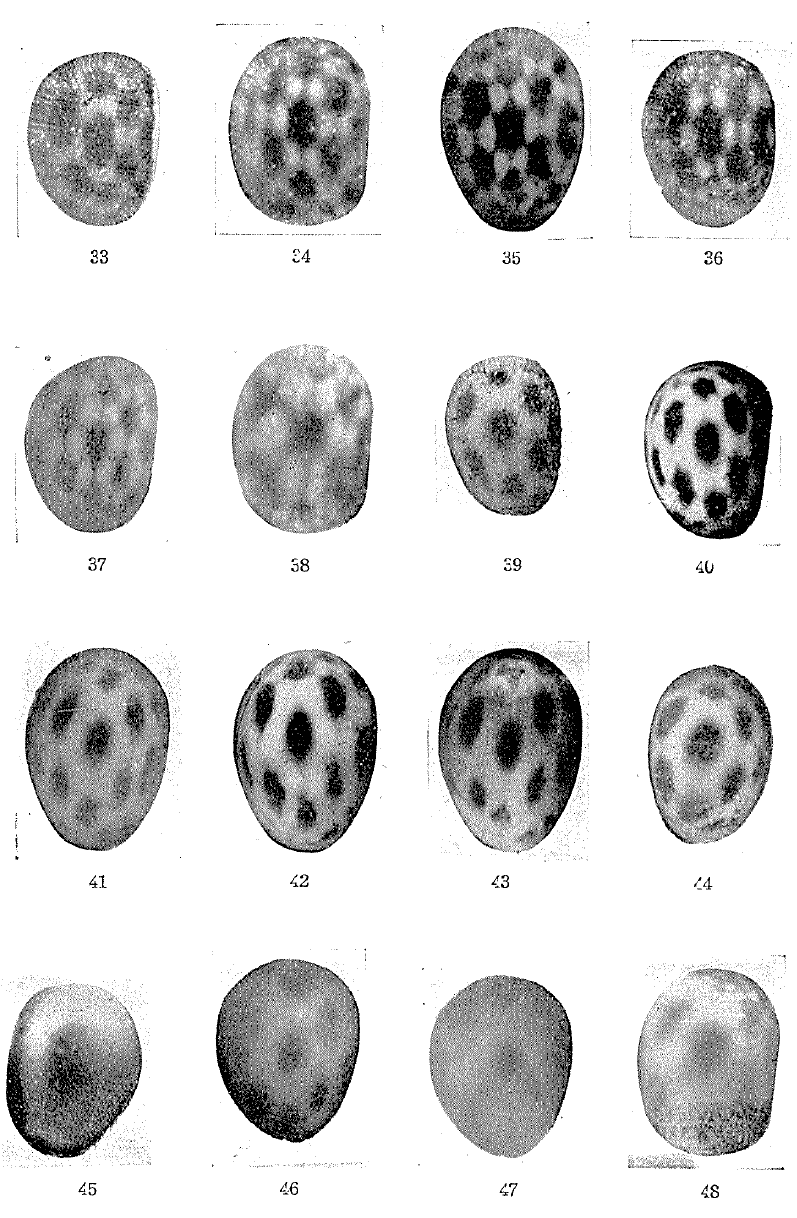
\includegraphics[width=4.5in]{./img/yagi1-hex-real.png}
  \caption{六角形の偽瞳孔(写真:\cite{yagi1951studies}より転載)}
  \label{FYagiHex}
\end{figure}

\begin{figure}[htbp]
  \centering
  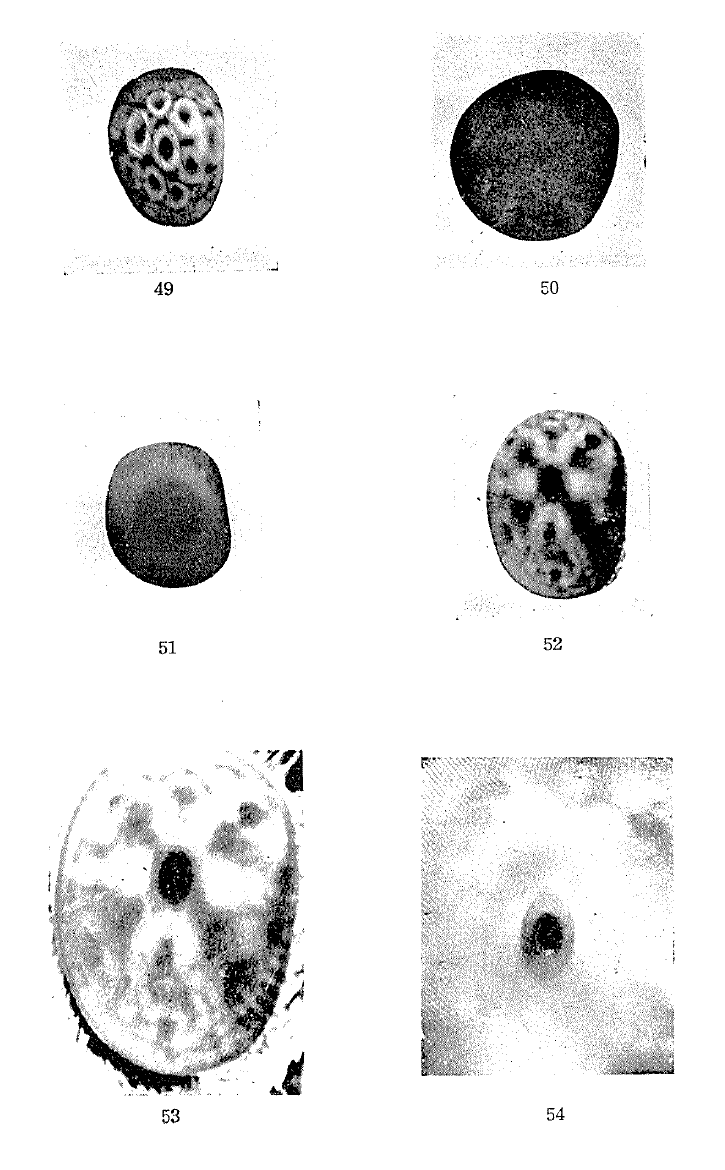
\includegraphics[width=4.5in]{./img/yagi1-ring-real.png}
  \caption{リング状の偽瞳孔(写真:\cite{yagi1951studies}より転載)}
  \label{FYagiRing}
\end{figure}


\newpage
\section{さまざまなオブジェクト}
\label{SVariousObject}

本手法はさまざまなオブジェクトに対して適用可能である。
以下にその例を示す。

\begin{figure}[htbp]
  \centering
\subfigure[図1]{
\includegraphics*[width=.45\columnwidth]{./img/screenshot/obj/shell/screenshot001.bmp}
\label{FShell1}}
\subfigure[図2]{
\includegraphics*[width=.45\columnwidth]{./img/screenshot/obj/shell/screenshot002.bmp}
\label{FShell2}}\\
\subfigure[図3]{
\includegraphics*[width=.45\columnwidth]{./img/screenshot/obj/shell/screenshot003.bmp}
\label{FShell3}}
\subfigure[図4]{
\includegraphics*[width=.45\columnwidth]{./img/screenshot/obj/shell/screenshot004.bmp}
\label{FShell4}}
  \caption{貝殻オブジェクトへの適用}
  \label{FShell}
\end{figure}

\begin{figure}[htbp]
  \centering
\subfigure[図1]{
\includegraphics*[width=.45\columnwidth]{./img/screenshot/obj/tori_head/screenshot001.bmp}
\label{FToriHead1}}
\subfigure[図2]{
\includegraphics*[width=.45\columnwidth]{./img/screenshot/obj/tori_head/screenshot002.bmp}
\label{FToriHead2}}\\
\subfigure[図3]{
\includegraphics*[width=.45\columnwidth]{./img/screenshot/obj/tori_head/screenshot003.bmp}
\label{FToriHead3}}
\subfigure[図4]{
\includegraphics*[width=.45\columnwidth]{./img/screenshot/obj/tori_head/screenshot004.bmp}
\label{FToriHead4}}
  \caption{鳥頭オブジェクトへの適用}
  \label{FToriHead}
\end{figure}


\section{応用事例}
\label{SKagoshima}

本研究の応用事例として、2014年12月11日から2014年12月14日の期間に行った「かごしまアートフェスタ2014」への展示の事例を紹介する。

「複眼的宇宙鳥 Bircco (バーコ)と探索する宇宙蜘蛛」と題して、鹿児島市「かごしま県民交流センター」においてアート作品として本手法を応用した展示を行った。
入力機器としてキネクト(Microsoft Kinect センサー)を使用しているため、観客は手を左右にかざすことにより作品中のオブジェクトを回転したり、視点の種類を変更することができる。
本研究では、映画やゲームなどのエンターテインメント分野においてリアリティを向上させるための技術として位置づけていたが、キネクトのようなインタラクティブ技術とを組み合わせることによって、視点の位置によって見え方が変わるという特性自体を活かした新たな研究の方向性を生み出すことができるのではないだろうか。

%% エンタメに貢献できることを考えていたが、展示を行って
%% 視線によって変化する外観と、キネクトのようなインタラクティブ技術とを組み合わせることによって、偽瞳孔の特性を体感的に

%% 映画とかは現実感を上げるための技術だけど、視点の位置によって見え方が変わるという特性自体を


\begin{figure}[htbp]
  \centering
\subfigure[図1]{
\includegraphics*[width=.45\columnwidth]{./img/bircco_green.jpg}
\label{FBirccoGreen}}
\subfigure[図2]{
\includegraphics*[width=.45\columnwidth]{./img/bircco_red.jpg}
\label{FBirccoRed}}\\
\subfigure[図1]{
\includegraphics*[width=.45\columnwidth]{./img/bircco_youjo1.jpg}
\label{FBirccoYoujo1}}
\subfigure[図2]{
\includegraphics*[width=.45\columnwidth]{./img/bircco_youjo2.jpg}
\label{FBirccoYoujo2}}
  \caption{複眼的宇宙鳥 Bircco (バーコ)と探索する宇宙蜘蛛}
  \label{FBircco}
\end{figure}










%--前書いてたやつ----------------------------------------------------------------------------------------
%% \newpage
%% \section{平面オブジェクトに適用した結果}
%% \label{SPlaneObject}

%% 本研究で提案した屈折を表現する手法の有用性を評価するため、平面オブジェクトに対して球体レンズを適用する実験を行った。


%% \begin{figure}[htbp]
%%   \centering
%% \subfigure[CAPTIONa]{
%% \includegraphics*[width=.45\columnwidth]{./img/single/screenshot001.bmp}
%% \label{F}}
%% \subfigure[CAPTIONb]{
%% \includegraphics*[width=.45\columnwidth]{./img/single/screenshot002.bmp}
%% \label{F}}\\
%% \subfigure[CAPTIONc]{
%% \includegraphics*[width=.45\columnwidth]{./img/single/screenshot003.bmp}
%% \label{F}}
%% \subfigure[CAPTIONd]{
%% \includegraphics*[width=.45\columnwidth]{./img/single/screenshot004.bmp}
%% \label{F}}\\
%% \subfigure[CAPTIONa]{
%% \includegraphics*[width=.45\columnwidth]{./img/single/screenshot005.bmp}
%% \label{F}}
%% \subfigure[CAPTIONb]{
%% \includegraphics*[width=.45\columnwidth]{./img/single/screenshot006.bmp}
%% \label{F}}\\
%%   \caption{CAPTION}
%%   \label{F}
%% \end{figure}

%% \begin{figure}[htbp]
%%   \centering
%% \subfigure[CAPTIONa]{
%% \includegraphics*[width=.45\columnwidth]{./img/single/screenshot007.bmp}
%% \label{F}}
%% \subfigure[CAPTIONb]{
%% \includegraphics*[width=.45\columnwidth]{./img/single/screenshot008.bmp}
%% \label{F}}\\
%% \subfigure[CAPTIONc]{
%% \includegraphics*[width=.45\columnwidth]{./img/single/screenshot009.bmp}
%% \label{F}}
%% \subfigure[CAPTIONd]{
%% \includegraphics*[width=.45\columnwidth]{./img/single/screenshot010.bmp}
%% \label{F}}\\
%% \subfigure[CAPTIONa]{
%% \includegraphics*[width=.45\columnwidth]{./img/single/screenshot011.bmp}
%% \label{F}}
%% \subfigure[CAPTIONb]{
%% \includegraphics*[width=.45\columnwidth]{./img/single/screenshot012.bmp}
%% \label{F}}\\
%%   \caption{CAPTION}
%%   \label{F}
%% \end{figure}
